\documentclass[aspectratio=169, 10pt]{beamer}
\usetheme{metropolis}
\usepackage{tikz}
\usetikzlibrary{calc, arrows.meta, shapes.geometric}

% ============================================================
% PRESENTATION META INFORMATION
% ============================================================
\title{Engineering Curves: Construction of Cycloid}
\subtitle{Rolling Circle Method with Tangent \& Normal}
\author{Gajavada Sanjeevkumar}
\date{}

% ============================================================
% METROPOLIS NUMBERING & NAVIGATION SETUP
% ============================================================
\metroset{numbering=none}
\setbeamertemplate{navigation symbols}{}

\setbeamercolor{custom footer}{
  fg=white,
  bg=black!80
}

\newcommand{\stepnum}{1}

% Clean, robust custom footer template with numbers only and navigation links
\setbeamertemplate{footline}{%
  \ifnum\value{framenumber}>1
    \leavevmode%
    \hbox{%
      \begin{beamercolorbox}[
        wd=\paperwidth,
        ht=3.2ex,
        dp=1.4ex,
        leftskip=0.5cm,
        rightskip=0.5cm
      ]{custom footer}%
        \tiny
        \insertauthor
        \quad|\quad
        \inserttitle
        \hfill
        \hyperlink{slide:title}{\beamerbutton{Top}}%
        \hyperlink{slide:prev}{\beamerbutton{Prev}}%
        \hyperlink{slide:next}{\beamerbutton{Next}}%
        \hyperlink{slide:end}{\beamerbutton{End}}%
        \quad
        \ifnum\value{framenumber}=2
          Problem Statement%
        \else
          \stepnum
        \fi
      \end{beamercolorbox}%
    }%
  \fi%
}

% ============================================================
% CUSTOM TIKZ STYLES & DEFINITIONS
% ============================================================
\tikzset{
  axis line/.style={thin, dash pattern=on 6pt off 2pt on 1.5pt off 2pt, black!75}, 
  directrix line/.style={ultra thick, magenta!90!black},
  construction line/.style={thin, blue!60!black},
  arc line/.style={thin, dashed, red!85!black},
  main curve/.style={ultra thick, magenta!90!black},
  tangent line/.style={thick, green!50!black},
  normal line/.style={thick, orange!80!black},
  label line/.style={stealth-, thin, black!70},
  dimension extension/.style={thin, solid, black!60},
  >=Stealth,
}

\newcommand{\drawLegendCard}[1]{
  \node[draw=gray!50, fill=white, rounded corners=4pt, inner sep=4pt, anchor=north east] at (21.85, 8.5) {
    \scriptsize
    \begin{tabular}{l@{\,$\rightarrow$\,}l}
      #1
    \end{tabular}
  };
}

\begin{document}

% ============================================================
% TITLE SLIDE (Frame 1)
% ============================================================
\begin{frame}[label=slide:title,plain]
  \titlepage
\end{frame}

% ============================================================
% PROBLEM STATEMENT (Frame 2)
% ============================================================
\begin{frame}[label=slide:prev,fragile]{Problem Statement}
  \vfill
  \begin{block}{Question}
    \vspace{0.8em}
    Draw a \textbf{cycloid} generated by a circle of diameter $D = 50\text{ mm}$ rolling along a straight base line for \textbf{one complete revolution} without slipping.
    \vspace{0.8em}

    Construct a \textbf{tangent} and a \textbf{normal} to the cycloid at any point $P$ located on the curve.
  \end{block}
  \vfill
\end{frame}

% ============================================================
% STEP 1: GENERATING CIRCLE & DIRECTING LINE
% ============================================================
\renewcommand{\stepnum}{1}
\foreach \stage in {1,2,3,4,5,6,7,8,9,10} {
  \begin{frame}[fragile]{Step 1: Draw Generating Circle \& Directing Line}{Radius of generating circle = 25 mm (Stage \stage/10)}
  \centering
  \begin{tikzpicture}[scale=0.45]
    \useasboundingbox (-4.5,-3.5) rectangle (22.5,8.0);
    \drawLegendCard{ \textbf{$C_0$} & Initial Center Point \\ \textbf{$AA'$} & Directing Line \\ \textbf{Axis} & Center Line }
    \coordinate (C0) at (0,3.0);
    \fill[red!80!black] (C0) circle (3.5pt) node[above right, font=\tiny] {$C_0$};
    \ifnum\stage>1 \draw[thick, blue!80!black] (C0) circle (3.0); \fi
    \ifnum\stage>2 \draw[<->, thin, cyan!80!black] (0,3.0) -- (0,0) node[midway, right] {\tiny $R=25\text{ mm}$}; \fi
    \ifnum\stage>3 \draw[directrix line] (0,0) node[below left] {\small $A$} -- (18.85,0) node[below right] {\small $A'$}; \fi
    \ifnum\stage>4 \draw[axis line] (0,3.0) -- (18.85,3.0) node[right] {\small $C_{12}$}; \fi
    \ifnum\stage>5 \draw[dimension extension] (0,0) -- (0,-2.2); \fi
    \ifnum\stage>6 \draw[dimension extension] (18.85,0) -- (18.85,-2.2); \fi
    \ifnum\stage>7 \draw[<->, red!80!black, thin] (0,-1.8) -- (18.85,-1.8) node[midway, fill=white] {\tiny $\pi D = 157\text{ mm}$}; \fi
    \ifnum\stage>8 \draw[thin, construction line] (0,0) -- (C0); \fi
  \end{tikzpicture}
  \end{frame}
}

% ============================================================
% STEP 2: DIVIDE CIRCLE INTO 12 PARTS
% ============================================================
\renewcommand{\stepnum}{2}
\foreach \divcount in {0,1,2,3,4,5,6,7,8,9,10,11,12} {
  \begin{frame}[fragile]{Step 2: Divide Generating Circle into 12 Equal Parts}{Radius of generating circle = 25 mm (Division \divcount/12)}
  \centering
  \begin{tikzpicture}[scale=0.45]
    \useasboundingbox (-4.5,-3.5) rectangle (22.5,8.0);
    \drawLegendCard{ \textbf{$AA'$} & Directing Line \\ \textbf{Axis Line} & Center Line \\ \textbf{$0\dots12$} & Circle Divisions }
    \draw[directrix line] (0,0) node[below left] {\small $A$} -- (18.85,0) node[below right] {\small $A'$};
    \draw[axis line] (0,3.0) -- (18.85,3.0) node[right] {\small $C_{12}$};
    \coordinate (C0) at (0,3.0);
    \fill[red!80!black] (C0) circle (3.5pt) node[above right, font=\tiny] {$C_0$};
    \draw[thick, blue!80!black] (C0) circle (3.0);
    \draw[thin, construction line] (0,0) -- (C0);
    \draw[dimension extension] (0,0) -- (0,-2.2);
    \draw[dimension extension] (18.85,0) -- (18.85,-2.2);
    \draw[<->, red!80!black, thin] (0,-1.8) -- (18.85,-1.8) node[midway, fill=white] {\tiny $\pi D = 157\text{ mm}$};
    \ifnum\divcount>0
      \foreach \d in {1,...,\divcount} {
        \draw[thin, cyan!60!black, solid] (C0) -- ++(-\d*30+90:3.0);
      }
    \fi
  \end{tikzpicture}
  \end{frame}
}

% ============================================================
% STEP 3: DIVIDE DIRECTING LINE
% ============================================================
\renewcommand{\stepnum}{3}
\foreach \dcount in {0,1,2,3,4,5,6,7,8,9,10,11,12} {
  \begin{frame}[fragile]{Step 3: Divide Directing Line using Line Division Method}{Radius of generating circle = 25 mm (Part \dcount/12)}
  \centering
  \begin{tikzpicture}[scale=0.45]
    \useasboundingbox (-4.5,-3.5) rectangle (22.5,8.0);
    \drawLegendCard{ \textbf{$AA'$} & Directing Line \\ \textbf{$A X$} & Inclined Line \\ \textbf{$1'\dots12'$} & Parallel Divisions }
    \draw[directrix line] (0,0) node[below left] {\small $A$} -- (18.85,0) node[below right] {\small $A'$};
    \draw[axis line] (0,3.0) -- (18.85,3.0) node[right] {\small $C_{12}$};
    \coordinate (C0) at (0,3.0);
    \fill[red!80!black] (C0) circle (3.5pt) node[above right, font=\tiny] {$C_0$};
    \draw[thick, blue!80!black] (C0) circle (3.0);
    \draw[thin, construction line] (0,0) -- (C0);
    \draw[dimension extension] (0,0) -- (0,-2.2);
    \draw[dimension extension] (18.85,0) -- (18.85,-2.2);
    \draw[<->, red!80!black, thin] (0,-1.8) -- (18.85,-1.8) node[midway, fill=white] {\tiny $\pi D = 157\text{ mm}$};
    \ifnum\dcount>0 \draw[thick, orange!80!black] (0,0) -- (17.38,-3.11) node[right, font=\tiny] {$X$}; \fi
  \end{tikzpicture}
  \end{frame}
}

% ============================================================
% STEP 4: PROJECT CENTERS C1..C12
% ============================================================
\renewcommand{\stepnum}{4}
\foreach \ccount in {0,1,2,3,4,5,6,7,8,9,10,11,12} {
  \begin{frame}[fragile]{Step 4: Project Divisions to Locate Centers $C_1\dots C_{12}$}{Radius of generating circle = 25 mm (Center \ccount/12)}
  \centering
  \begin{tikzpicture}[scale=0.45]
    \useasboundingbox (-4.5,-3.5) rectangle (22.5,8.0);
    \drawLegendCard{ \textbf{$AA'$} & Directing Line \\ \textbf{Axis Line} & Center Line \\ \textbf{$C_1\dots C_{12}$} & Center Points }
    \draw[directrix line] (0,0) node[below left] {\small $A$} -- (18.85,0) node[below right] {\small $A'$};
    \draw[axis line] (0,3.0) -- (18.85,3.0);
    \coordinate (C0) at (0,3.0);
    \fill[red!80!black] (C0) circle (3.5pt);
    \draw[thick, blue!80!black] (C0) circle (3.0);
    \draw[thin, construction line] (0,0) -- (C0);
    \draw[dimension extension] (0,0) -- (0,-2.2);
    \draw[dimension extension] (18.85,0) -- (18.85,-2.2);
    \draw[<->, red!80!black, thin] (0,-1.8) -- (18.85,-1.8) node[midway, fill=white] {\tiny $\pi D = 157\text{ mm}$};
    \ifnum\ccount>0
      \foreach \k in {1,...,\ccount} {
        \fill[red!80!black] ({\k*1.5708}, 3.0) circle (2.5pt);
      }
    \fi
  \end{tikzpicture}
  \end{frame}
}

% ============================================================
% STEP 5: DRAW HORIZONTAL REFERENCE LINES
% ============================================================
\renewcommand{\stepnum}{5}
\foreach \hcount in {0,1,2,3,4,5,6} {
  \begin{frame}[fragile]{Step 5: Draw Horizontal Reference Lines}{Radius of generating circle = 25 mm (Reference \hcount/6)}
  \centering
  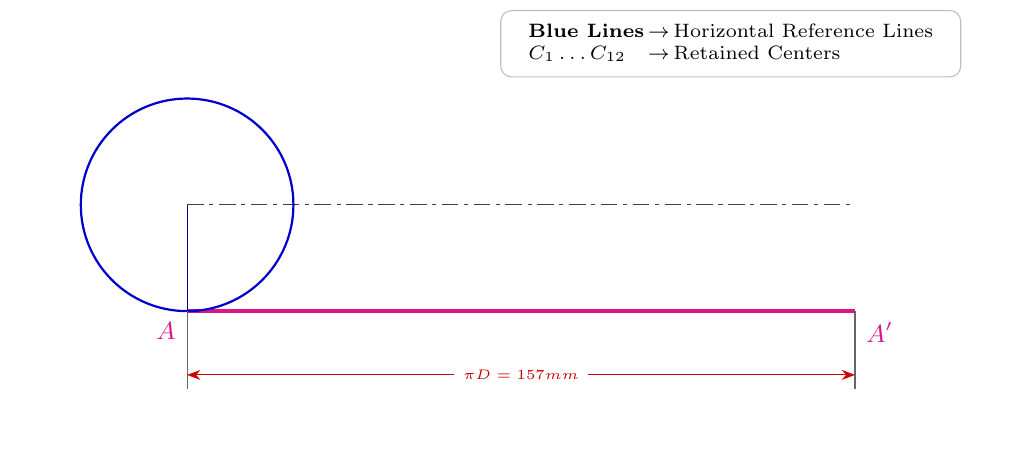
\begin{tikzpicture}[scale=0.45]
    \useasboundingbox (-4.5,-3.5) rectangle (22.5,8.0);
    \drawLegendCard{ \textbf{Blue Lines} & Horizontal Reference Lines \\ \textbf{$C_1\dots C_{12}$} & Retained Centers }
    \draw[directrix line] (0,0) node[below left] {\small $A$} -- (18.85,0) node[below right] {\small $A'$};
    \draw[axis line] (0,3.0) -- (18.85,3.0);
    \coordinate (C0) at (0,3.0); \draw[thick, blue!80!black] (C0) circle (3.0);
    \draw[thin, construction line] (0,0) -- (C0);
    \draw[dimension extension] (0,0) -- (0,-2.2);
    \draw[dimension extension] (18.85,0) -- (18.85,-2.2);
    \draw[<->, red!80!black, thin] (0,-1.8) -- (18.85,-1.8) node[midway, fill=white] {\tiny $\pi D = 157\text{ mm}$};
  \end{tikzpicture}
  \end{frame}
}

% ============================================================
% STEP 6: STRIKE CUTTING ARCS P0..P12
% ============================================================
\renewcommand{\stepnum}{6}
\foreach \pcount in {0,1,2,3,4,5,6,7,8,9,10,11,12} {
  \begin{frame}[fragile]{Step 6: Strike Cutting Arcs (Radius = 25 mm) to Locate Points}{Radius of generating circle = 25 mm (Point P\pcount)}
  \centering
  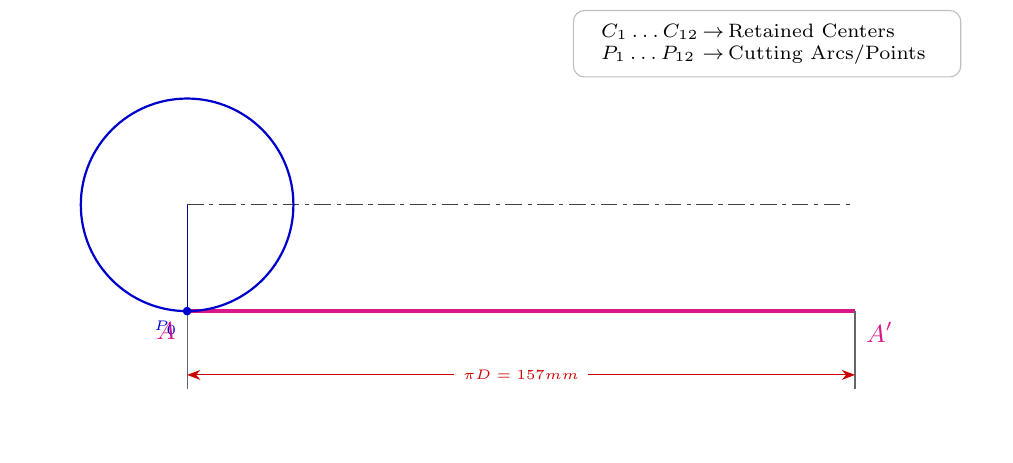
\begin{tikzpicture}[scale=0.45]
    \useasboundingbox (-4.5,-3.5) rectangle (22.5,8.0);
    \drawLegendCard{ \textbf{$C_1\dots C_{12}$} & Retained Centers \\ \textbf{$P_1\dots P_{12}$} & Cutting Arcs/Points }
    \draw[directrix line] (0,0) node[below left] {\small $A$} -- (18.85,0) node[below right] {\small $A'$};
    \draw[axis line] (0,3.0) -- (18.85,3.0);
    \coordinate (C0) at (0,3.0); \draw[thick, blue!80!black] (C0) circle (3.0);
    \draw[thin, construction line] (0,0) -- (C0);
    \draw[dimension extension] (0,0) -- (0,-2.2);
    \draw[dimension extension] (18.85,0) -- (18.85,-2.2);
    \draw[<->, red!80!black, thin] (0,-1.8) -- (18.85,-1.8) node[midway, fill=white] {\tiny $\pi D = 157\text{ mm}$};
    \fill[blue!80!black] (0,0) circle (3.5pt) node[below left, font=\tiny] {$P_0$};
  \end{tikzpicture}
  \end{frame}
}

% ============================================================
% STEP 7: JOIN POINTS TO FORM CYCLOID
% ============================================================
\renewcommand{\stepnum}{7}
\begin{frame}[fragile]{Step 7: Smoothly Join Points to Form Cycloid Curve}{Radius of generating circle = 25 mm - Plotting Points}
\centering
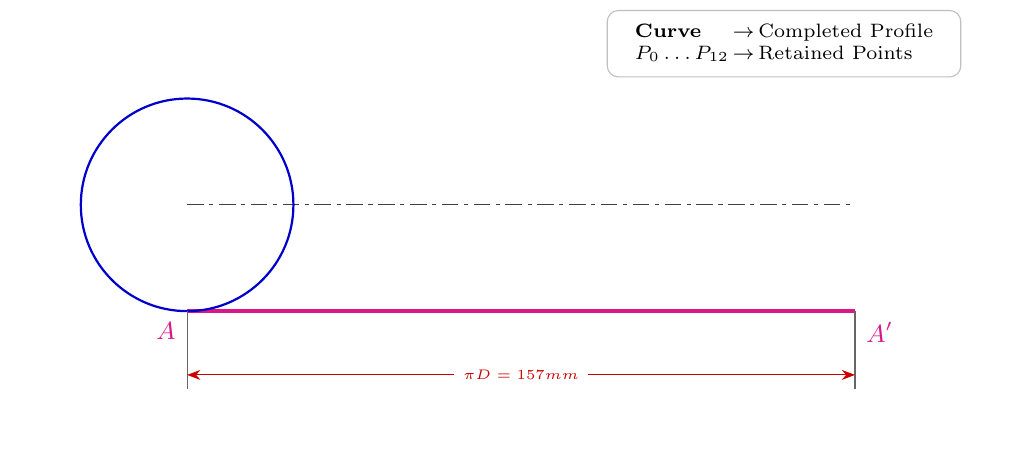
\begin{tikzpicture}[scale=0.45]
  \useasboundingbox (-4.5,-3.5) rectangle (22.5,8.0);
  \drawLegendCard{ \textbf{Curve} & Completed Profile \\ \textbf{$P_0\dots P_{12}$} & Retained Points }
  \draw[directrix line] (0,0) node[below left] {\small $A$} -- (18.85,0) node[below right] {\small $A'$};
  \draw[axis line] (0,3.0) -- (18.85,3.0);
  \coordinate (C0) at (0,3.0); \draw[thick, blue!80!black] (C0) circle (3.0);
  \draw[dimension extension] (0,0) -- (0,-2.2);
  \draw[dimension extension] (18.85,0) -- (18.85,-2.2);
  \draw[<->, red!80!black, thin] (0,-1.8) -- (18.85,-1.8) node[midway, fill=white] {\tiny $\pi D = 157\text{ mm}$};
\end{tikzpicture}
\end{frame}

\begin{frame}[fragile]{Step 7: Smoothly Join Points to Form Cycloid Curve}{Radius of generating circle = 25 mm - Final Curve}
\centering
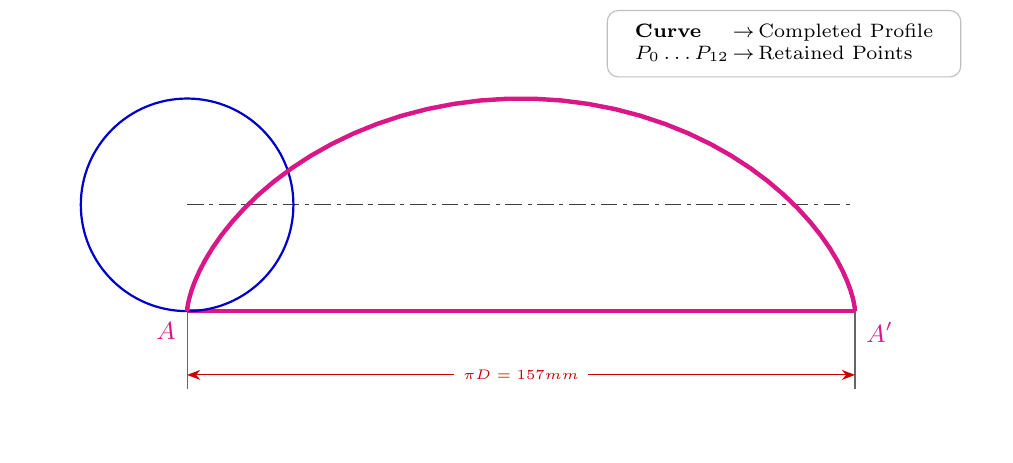
\begin{tikzpicture}[scale=0.45]
  \useasboundingbox (-4.5,-3.5) rectangle (22.5,8.0);
  \drawLegendCard{ \textbf{Curve} & Completed Profile \\ \textbf{$P_0\dots P_{12}$} & Retained Points }
  \draw[directrix line] (0,0) node[below left] {\small $A$} -- (18.85,0) node[below right] {\small $A'$};
  \draw[axis line] (0,3.0) -- (18.85,3.0);
  \coordinate (C0) at (0,3.0); \draw[thick, blue!80!black] (C0) circle (3.0);
  \draw[dimension extension] (0,0) -- (0,-2.2);
  \draw[dimension extension] (18.85,0) -- (18.85,-2.2);
  \draw[<->, red!80!black, thin] (0,-1.8) -- (18.85,-1.8) node[midway, fill=white] {\tiny $\pi D = 157\text{ mm}$};
  \draw[main curve, samples=50, domain=0:6.28318] plot ({3*(\x - sin(\x r))}, {3*(1 - cos(\x r))});
\end{tikzpicture}
\end{frame}

% ============================================================
% STEP 8: TANGENT & NORMAL CONSTRUCTION
% ============================================================
\renewcommand{\stepnum}{8}

\begin{frame}[fragile]{Step 8: Constructing Tangent and Normal}{Radius = 25 mm - Locate Point $P$}
\centering
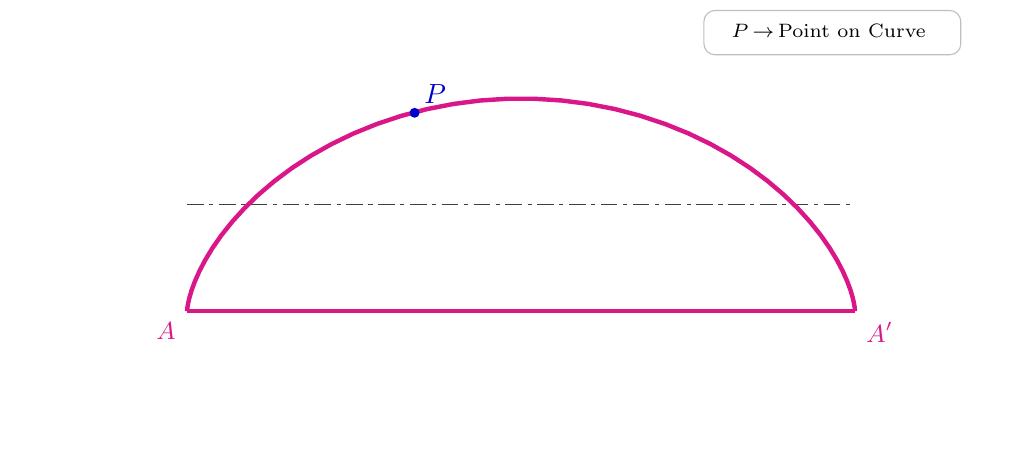
\begin{tikzpicture}[scale=0.45]
  \useasboundingbox (-4.5,-3.5) rectangle (22.5,8.0);
  \drawLegendCard{ \textbf{$P$} & Point on Curve }
  \draw[directrix line] (0,0) node[below left] {\small $A$} -- (18.85,0) node[below right] {\small $A'$};
  \draw[axis line] (0,3.0) -- (18.85,3.0);
  \draw[main curve, samples=50, domain=0:6.28318] plot ({3*(\x - sin(\x r))}, {3*(1 - cos(\x r))});
  \coordinate (P) at (6.42, 5.598);
  \fill[blue!80!black] (P) circle (4pt) node[above right] {$P$};
\end{tikzpicture}
\end{frame}

\begin{frame}[fragile]{Step 8: Constructing Tangent and Normal}{Radius = 25 mm - Locate Center $C_p$}
\centering
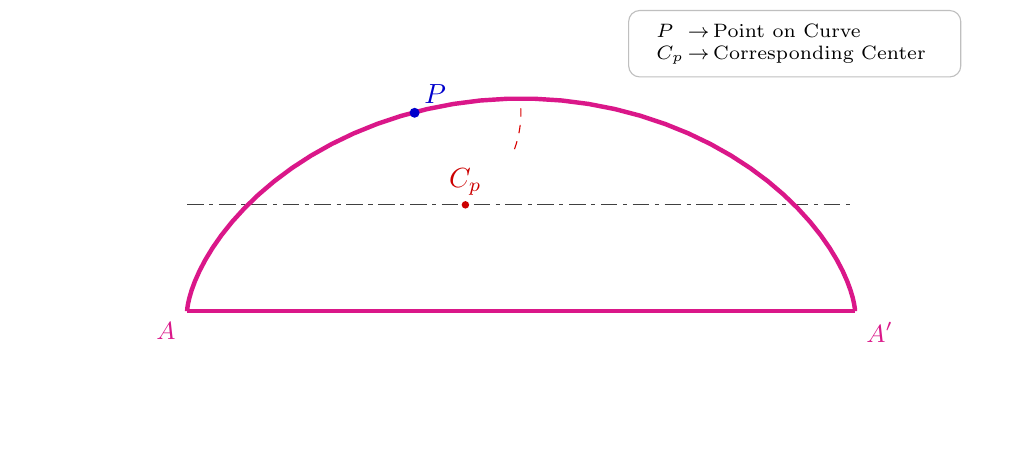
\begin{tikzpicture}[scale=0.45]
  \useasboundingbox (-4.5,-3.5) rectangle (22.5,8.0);
  \drawLegendCard{ \textbf{$P$} & Point on Curve \\ \textbf{$C_p$} & Corresponding Center }
  \draw[directrix line] (0,0) node[below left] {\small $A$} -- (18.85,0) node[below right] {\small $A'$};
  \draw[axis line] (0,3.0) -- (18.85,3.0);
  \draw[main curve, samples=50, domain=0:6.28318] plot ({3*(\x - sin(\x r))}, {3*(1 - cos(\x r))});
  \coordinate (P) at (6.42, 5.598);
  \fill[blue!80!black] (P) circle (4pt) node[above right] {$P$};
  \coordinate (Cp) at (7.8540, 3.0);
  \fill[red!80!black] (Cp) circle (3pt) node[above] {$C_p$};
  \draw[arc line] (P) ++(-20:3.0) arc (-20:5:3.0);
\end{tikzpicture}
\end{frame}

\begin{frame}[fragile]{Step 8: Constructing Tangent and Normal}{Radius = 25 mm - Radius Vector $P-C_p$}
\centering
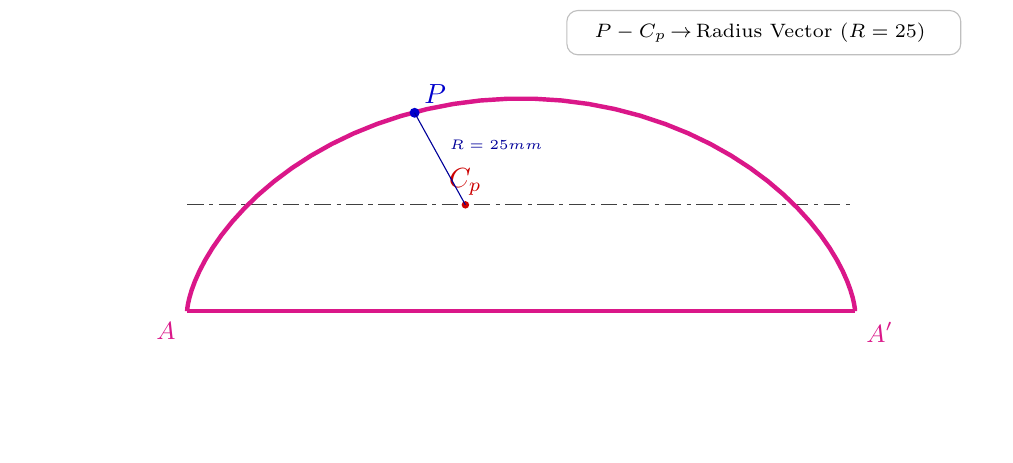
\begin{tikzpicture}[scale=0.45]
  \useasboundingbox (-4.5,-3.5) rectangle (22.5,8.0);
  \drawLegendCard{ \textbf{$P-C_p$} & Radius Vector ($R=25$) }
  \draw[directrix line] (0,0) node[below left] {\small $A$} -- (18.85,0) node[below right] {\small $A'$};
  \draw[axis line] (0,3.0) -- (18.85,3.0);
  \draw[main curve, samples=50, domain=0:6.28318] plot ({3*(\x - sin(\x r))}, {3*(1 - cos(\x r))});
  \coordinate (P) at (6.42, 5.598);
  \coordinate (Cp) at (7.8540, 3.0);
  \fill[blue!80!black] (P) circle (4pt) node[above right] {$P$};
  \fill[red!80!black] (Cp) circle (3pt) node[above] {$C_p$};
  \draw[construction line] (P) -- (Cp) node[midway, above right, font=\tiny] {$R=25\text{ mm}$};
\end{tikzpicture}
\end{frame}

\begin{frame}[fragile]{Step 8: Constructing Tangent and Normal}{Radius = 25 mm - Normal Line $N-N'$}
\centering
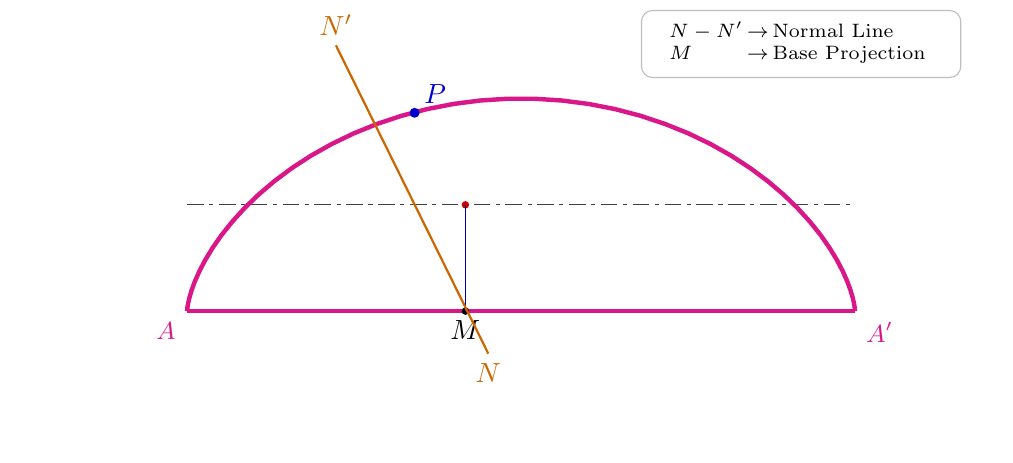
\begin{tikzpicture}[scale=0.45]
  \useasboundingbox (-4.5,-3.5) rectangle (22.5,8.0);
  \drawLegendCard{ \textbf{$N-N'$} & Normal Line \\ \textbf{$M$} & Base Projection }
  \draw[directrix line] (0,0) node[below left] {\small $A$} -- (18.85,0) node[below right] {\small $A'$};
  \draw[axis line] (0,3.0) -- (18.85,3.0);
  \draw[main curve, samples=50, domain=0:6.28318] plot ({3*(\x - sin(\x r))}, {3*(1 - cos(\x r))});
  \coordinate (P) at (6.42, 5.598);
  \coordinate (Cp) at (7.8540, 3.0);
  \coordinate (M) at (7.8540, 0);
  \fill[blue!80!black] (P) circle (4pt) node[above right] {$P$};
  \fill[red!80!black] (Cp) circle (3pt);
  \fill[black] (M) circle (3pt) node[below] {$M$};
  \draw[construction line, solid] (Cp) -- (M);
  \draw[normal line] (8.5, -1.2) node[below] {$N$} -- (4.2, 7.5) node[above] {$N'$};
\end{tikzpicture}
\end{frame}

\begin{frame}[fragile]{Step 8: Constructing Tangent and Normal}{Radius = 25 mm - Tangent Line $T-T'$ & Final Result}
\centering
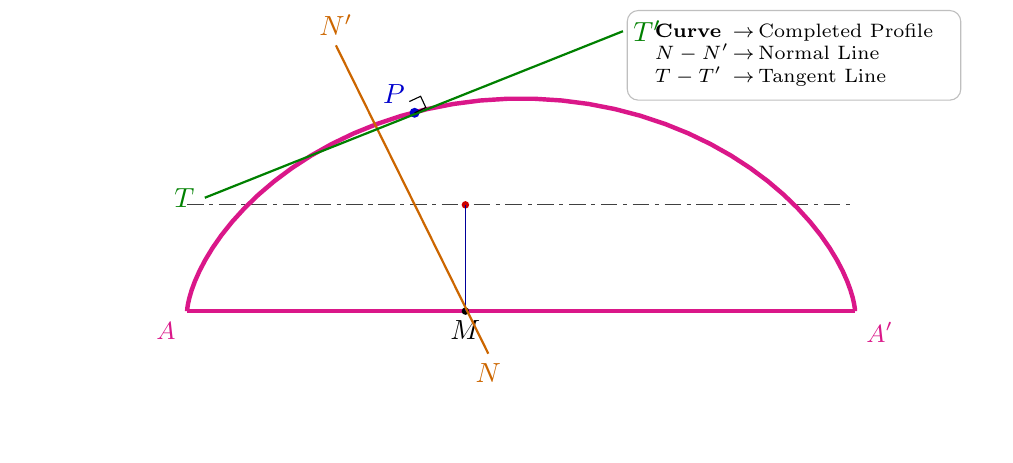
\begin{tikzpicture}[scale=0.45]
  \useasboundingbox (-4.5,-3.5) rectangle (22.5,8.0);
  \drawLegendCard{ \textbf{Curve} & Completed Profile \\ \textbf{$N-N'$} & Normal Line \\ \textbf{$T-T'$} & Tangent Line }
  \draw[directrix line] (0,0) node[below left] {\small $A$} -- (18.85,0) node[below right] {\small $A'$};
  \draw[axis line] (0,3.0) -- (18.85,3.0);
  \draw[main curve, samples=50, domain=0:6.28318] plot ({3*(\x - sin(\x r))}, {3*(1 - cos(\x r))});
  \coordinate (P) at (6.42, 5.598);
  \coordinate (Cp) at (7.8540, 3.0);
  \coordinate (M) at (7.8540, 0);
  \fill[blue!80!black] (P) circle (4pt) node[above left] {$P$};
  \fill[red!80!black] (Cp) circle (3pt);
  \fill[black] (M) circle (3pt) node[below] {$M$};
  \draw[construction line, solid] (Cp) -- (M);
  \draw[normal line] (8.5, -1.2) node[below] {$N$} -- (4.2, 7.5) node[above] {$N'$};
  \draw[tangent line] (0.5, 3.2) node[left] {$T$} -- (12.3, 7.9) node[right] {$T'$};
  
  \begin{scope}[shift={(6.42, 5.598)}, rotate=25]
    \draw[thin, black] (0,0) -- (0.35,0) -- (0.35,0.35) -- (0,0.35);
  \end{scope}
\end{tikzpicture}
\end{frame}

% ============================================================
% STEP 9: SUMMARY & VERIFICATION
% ============================================================
\renewcommand{\stepnum}{9}

\begin{frame}[fragile]{Step 9: Summary \& Verification}{Reviewing Construction Steps}
\begin{itemize}
    \item Constructed rolling generating circle of diameter $D = 50\text{ mm}$ ($R = 25\text{ mm}$).
    \item Calculated and projected baseline length $\pi D = 157\text{ mm}$.
    \item Divided circle and base line into 12 equal parts using line division method.
\end{itemize}
\end{frame}

\begin{frame}[fragile]{Step 9: Summary \& Verification}{Tracing Locus Points}
\begin{itemize}
    \item Projected center points $C_1$ through $C_{12}$ along the horizontal center path line.
    \item Struck cutting arcs of radius $R = 25\text{ mm}$ from each center to locate points $P_1$ through $P_{12}$.
    \item Joined all points smoothly to form the complete cycloid curve.
\end{itemize}
\end{frame}

\begin{frame}[fragile]{Step 9: Summary \& Verification}{Tangent \& Normal Principles}
\begin{itemize}
    \item Located target point $P$ on the curve and identified its corresponding center $C_p$.
    \item Dropped perpendicular from $C_p$ to base line $AA'$ to find point of contact $M$.
    \item Established normal line $P-M$ and constructed perpendicular tangent $T-T'$.
\end{itemize}
\end{frame}

\begin{frame}[fragile]{Step 9: Summary \& Verification}{Engineering Drawing Standards}
\begin{itemize}
    \item Ensured clean line weighting distinguishing construction lines from final curves.
    \item Verified dimensional accuracy and symmetry around the apex $P_6$.
\end{itemize}
\end{frame}

\begin{frame}[label=slide:next,fragile]{Step 9: Summary \& Verification}{Final Quality Control Check}
\begin{itemize}
    \item All required parameters and labels properly displayed in drawing legend cards.
    \item Ready for final presentation and sheet layout transfer.
\end{itemize}
\end{frame}

% ============================================================
% CONCLUSION
% ============================================================
\renewcommand{\stepnum}{10}

\begin{frame}[fragile]{Conclusion}{Key Takeaways}
\begin{itemize}
    \item Cycloid curves play a vital role in mechanical engineering and gear design.
    \item The rolling circle method provides precise geometric locus generation.
\end{itemize}
\end{frame}

\begin{frame}[fragile]{Conclusion}{Applications in Mechanisms}
\begin{itemize}
    \item Application in cycloidal tooth profiles ensuring smooth power transmission.
    \item Understanding instantaneous centers simplifies tangent and normal construction.
\end{itemize}
\end{frame}

\begin{frame}[fragile]{Conclusion}{Q \& A}
\begin{itemize}
    \item Open floor for questions and technical clarifications.
\end{itemize}
\end{frame}

\begin{frame}[label=slide:end,fragile]{Conclusion}{End of Presentation}
\centering
\Large Thank You! \\
\vspace{1em}
\normalsize Department of Mechanical Engineering \\
Gajavada Sanjeevkumar
\end{frame}

end{document}
